\documentclass[12pt]{article}
\usepackage[english]{babel}
\usepackage{natbib}
\usepackage{url}
\usepackage[utf8x]{inputenc}
\usepackage{amsmath}
\usepackage{graphicx}
\graphicspath{{Images/}}
\usepackage{parskip}
\usepackage{fancyhdr}
\usepackage{vmargin}
\setmarginsrb{3 cm}{2.5 cm}{3 cm}{2.5 cm}{1 cm}{1.5 cm}{1 cm}{1.5 cm}

\title{El atractor de Lorenz, Ejemplo de caos dinámico}								% Title
\author{Martha Anahí Iñiguez Beltrán}						% Author
\date{\today}											% Date

\makeatletter
\let\thetitle\@title
\let\theauthor\@author
\let\thedate\@date
\makeatother

\pagestyle{fancy}
\fancyhf{}
\rhead{Física Computacional}
\lhead{\thetitle}
\cfoot{\thepage}

\begin{document}

\begin{titlepage}
\centering
    \vspace*{0.5 cm}
    
\includegraphics[width=5cm]{unison.jpg}\\[1.0 cm]	% University Logo
    \textsc{\LARGE Universidad de Sonora}\\[2.0 cm]	% University Name
    \textsc{\Large Departamento de ciencias exactas}\\[1.0 cm]
\textsc{\Large Física Computacional}\\[0.5 cm]
\rule{\linewidth}{0.2 mm} \\[0.4 cm]
{ \huge \bfseries \thetitle}\\
\rule{\linewidth}{0.2 mm} \\[1.5 cm]
\begin{minipage}{0.6\textwidth}
\begin{flushleft} \large
\emph{Alumno:}\\
\theauthor
\end{flushleft}
\end{minipage}~
\begin{minipage}{0.4\textwidth}
\begin{flushright} \large
214202804
\end{flushright}
\end{minipage}\\[2 cm]


{\large \thedate}\\[2 cm]

\vfill

\end{titlepage}

\tableofcontents
\pagebreak


\section{Introducción}
\noindent

En 1963, Edward Lorenz (1917-2008), quien se interesaba en el problema de la convección en la atmósfera terrestre, simplificó de forma drástica las ecuaciones de Navier-Stokes de la mecánica de fluidos, conocidas por su complejidad. El modelo atmosférico de Lorenz es lo que los físicos llaman un modelo de juguete: aunque probablemente no corresponda con la realidad, Lorenz no tardó mucho en darse cuenta que era un modelo matemático muy interesante. Las ecuaciones de Lorenz dependen de tres números x, y y z, de manera que cada punto del espacio (x,y,z) representa un estado de la atmósfera y para estudiar su evolución hay que seguir un campo de vectores.

\section{Código}

El código empleado para desarrollar cada unas de las visualizaciones y animaciones queda expuesto a continuación. Nótese que se muestra el código de ejemplo de una sola visualización y una animación.

\subsection{Visualización}

\begin{verbatim}
%matplotlib inline
import numpy as np, matplotlib.pyplot as plt, matplotlib.font_manager as fm, os
from scipy.integrate import odeint
from mpl_toolkits.mplot3d.axes3d import Axes3D

font_family = 'Myriad Pro'
title_font = fm.FontProperties(family=font_family, style='normal', size=20, weight='normal', stretch='normal')

save_folder = 'images'
if not os.path.exists(save_folder):
    os.makedirs(save_folder)

# Definimos el estado inicial del sistema (x, y, z posiciones en el espacio)
initial_state = [0.1, 0, 0]

#Definimos los parametro sigma, rho y beta del sistema
sigma = 10.
rho   = 28.
beta  = 8./3.

# Definimos los puntos de tiempo a resolver espaciados uniformemente entre tiempo inicial y final.
start_time = 0
end_time = 100
time_points = np.linspace(start_time, end_time, end_time*100)

# Definimos el sistema de Lorenz
# x, y, yz componen el estado del sistema, t es el tiempo, y sigma, rho, beta son los parámetros del sistema
def lorenz_system(current_state, t):
    
    # posiciones de x, y, z en el espacio en el tiempo actual
    x, y, z = current_state
    
    # definir las 3 ecuaciones diferenciales ordinarias conocidas como las ecuaciones de Lorenz
    dx_dt = sigma * (y - x)
    dy_dt = x * (rho - z) - y
    dz_dt = x * y - beta * z
    
    # devolver una lista de las ecuaciones que describen el sistema
    return [dx_dt, dy_dt, dz_dt]
    
    # Usa odeint () para resolver un sistema de ecuaciones diferenciales ordinarias
# los argumentos son:
# 1, una función - calcula las derivadas
# 2, un vector de condiciones iniciales del sistema (también conocido como #posiciones x, y, z en el espacio)
# 3, una secuencia de puntos de tiempo para resolver
# devuelve una matriz de matrices de valores x, y y z para cada punto de tiempo, con los valores iniciales en la primera fila
xyz = odeint(lorenz_system, initial_state, time_points)

# extraer las matrices individuales de los valores x, y y z de la matriz de matrices
x = xyz[:, 0]
y = xyz[:, 1]
z = xyz[:, 2]

# trazar el atractor Lorenz en el espacio de fase tridimensional
fig = plt.figure(figsize=(12, 9))
ax = fig.gca(projection='3d')
ax.xaxis.set_pane_color((1,1,1,1))
ax.yaxis.set_pane_color((1,1,1,1))
ax.zaxis.set_pane_color((1,1,1,1))
ax.plot(x, y, z, color='g', alpha=0.7, linewidth=0.6)
ax.set_title('Lorenz attractor phase diagram', fontproperties=title_font)

fig.savefig('{}/lorenz-attractor-3d.png'.format(save_folder), dpi=180, bbox_inches='tight')
plt.show()

# ahora trazar cortes bidimensionales del espacio de fase tridimensional
fig, ax = plt.subplots(1, 3, sharex=False, sharey=False, figsize=(17, 6))

# graficar los valores x vs y
ax[0].plot(x, y, color='r', alpha=0.7, linewidth=0.3)
ax[0].set_title('x-y phase plane', fontproperties=title_font)

# graficar los valores x vs z
ax[1].plot(x, z, color='m', alpha=0.7, linewidth=0.3)
ax[1].set_title('x-z phase plane', fontproperties=title_font)

# graficar los valores y vs z
ax[2].plot(y, z, color='b', alpha=0.7, linewidth=0.3)
ax[2].set_title('y-z phase plane', fontproperties=title_font)

fig.savefig('{}/lorenz-attractor-phase-plane.png'.format(save_folder), dpi=180, bbox_inches='tight')
plt.show()

# graficar la solución que se generó
from numpy import loadtxt
from pylab import figure, plot, xlabel, grid, hold, legend, title, savefig
from matplotlib.font_manager import FontProperties
%matplotlib inline 

figure(1, figsize=(10, 6))

xlabel('t')
grid(True)
hold(True)
lw = 1

plot(time_points, x, 'm', linewidth=lw)
plot(time_points, y, 'b', linewidth=lw)
plot(time_points, z, 'r', linewidth=lw)

legend((r'$x$', r'$y$', r'$z$'), prop=FontProperties(size=16))
title('Evolución de condición inicial/en función del tiempo')
savefig('Evolución 1.png', dpi=100)

\end{verbatim}

\subsection{Animación}

\begin{verbatim}
%matplotlib inline
import numpy as np, matplotlib.pyplot as plt, glob, os
import IPython.display as IPdisplay, matplotlib.font_manager as fm
from scipy.integrate import odeint
from mpl_toolkits.mplot3d.axes3d import Axes3D
from PIL import Image

# define las fuentes para usar en las gráficas
family = 'Myriad Pro'
title_font = fm.FontProperties(family=family, style='normal', size=20, weight='normal', stretch='normal')

save_folder = 'images/lorenz-animate'
if not os.path.exists(save_folder):
    os.makedirs(save_folder)

# definir el estado inicial del sistema (posiciones x, y, z en el espacio)
initial_state = [0.1, 0, 0]

# definir los parametros sigma, rho, y beta del sistema
sigma = 10.
rho   = 28.
beta  = 8./3.

# Definimos los puntos de tiempo a resolver espaciados uniformemente entre tiempo inicial y final.
start_time = 1
end_time = 60
interval = 100
time_points = np.linspace(start_time, end_time, end_time * interval)

# definir el sistema de Lorenz
def lorenz_system(current_state, t):
    x, y, z = current_state
    dx_dt = sigma * (y - x)
    dy_dt = x * (rho - z) - y
    dz_dt = x * y - beta * z
    return [dx_dt, dy_dt, dz_dt]

# graficar el sistema en 3 di
def plot_lorenz(xyz, n):
    fig = plt.figure(figsize=(12, 9))
    ax = fig.gca(projection='3d')
    ax.xaxis.set_pane_color((1,1,1,1))
    ax.yaxis.set_pane_color((1,1,1,1))
    ax.zaxis.set_pane_color((1,1,1,1))
    x = xyz[:, 0]
    y = xyz[:, 1]
    z = xyz[:, 2]
    ax.plot(x, y, z, color='g', alpha=0.7, linewidth=0.7)
    ax.set_xlim((-30,30))
    ax.set_ylim((-30,30))
    ax.set_zlim((0,50))
    ax.set_title('Lorenz system attractor', fontproperties=title_font)
    
    plt.savefig('{}/{:03d}.png'.format(save_folder, n), dpi=60, bbox_inches='tight', pad_inches=0.1)
    plt.close()

# devolver una lista en trozos iterativamente más grandes
def get_chunks(full_list, size):
    size = max(1, size)
    chunks = [full_list[0:i] for i in range(1, len(full_list) + 1, size)]
    return chunks

# # obtener trozos cada vez más grandes de los puntos de tiempo, para revelar el atractor un cuadro a la vez
chunks = get_chunks(time_points, size=20)

#obtener los puntos para graficar, un pedazo de tiempo a la vez, integrando el sistema de ecuaciones
points = [odeint(lorenz_system, initial_state, chunk) for chunk in chunks]

# graficar cada conjunto de puntos, uno a la vez, guardando cada gráfica
for n, point in enumerate(points):
    plot_lorenz(point, n)

# crear una lista de duraciones de visualización, una para cada fotograma
first_last = 100 #show the first and last frames for 100 ms
standard_duration = 5 #show all other frames for 5 ms
durations = tuple([first_last] + [standard_duration] * (len(points) - 2) + [first_last])

# cargar todas las imágenes estáticas en una lista
images = [Image.open(image) for image in glob.glob('{}/*.png'.format(save_folder))]
gif_filepath = 'images/animated-lorenz-attractor.gif'

# guardar como un gif animado
gif = images[0]
gif.info['duration'] = durations #ms per frame
gif.info['loop'] = 0 #how many times to loop (0=infinite)
gif.save(fp=gif_filepath, format='gif', save_all=True, append_images=images[1:])

# verificar que la cantidad de cuadros en el gif sea igual a la cantidad de archivos de imagen y duraciones
Image.open(gif_filepath).n_frames == len(images) == len(durations)

IPdisplay.Image(url=gif_filepath)

\end{verbatim}

\section{Resultados}

A continuacion se muestran los resultados obtenidos de las visualizaciones. El gif será incluido en la carpeta con los archivos generados con nuestro código.

\subsection{Sigma=10, Beta=8/3, Rho=28}

\begin{figure}
\begin{centering}
  \includegraphics[scale = 0.5]{lorenz-attractor-3d.png}
  \caption{Atractor de Lorenz}
\end{centering}
\end{figure}

\begin{figure}
\begin{centering}
  \includegraphics[scale = 0.4]{lorenz-attractor-phase-plane.png}
  \caption{Vista de los planos ortogonales del atractor de 2D}
\end{centering}
\end{figure}

\begin{figure}
\begin{centering}
  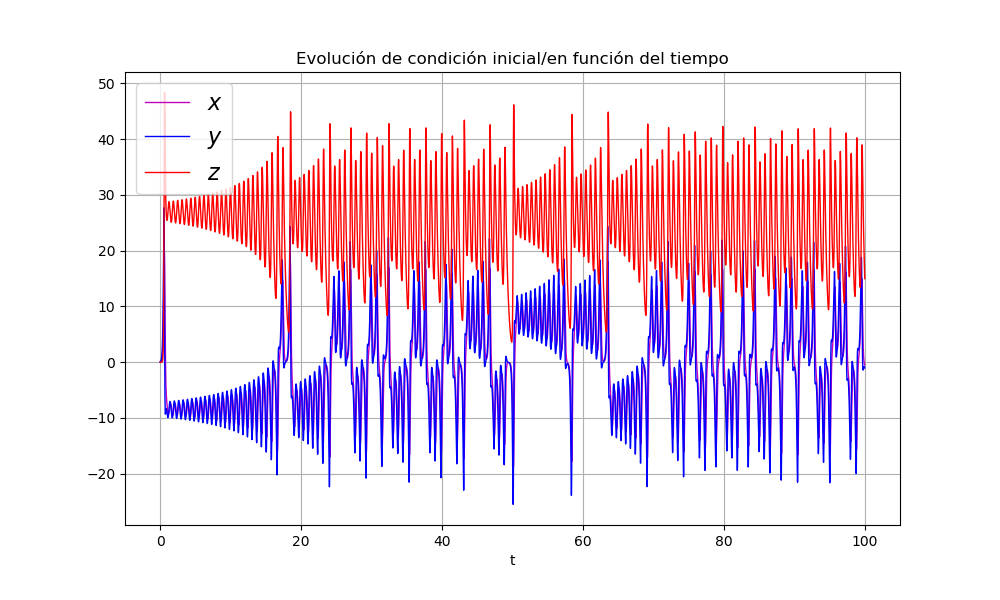
\includegraphics[scale = 0.65]{Evolucion1.png}
  \caption{Evolucion de cada variable respecto al tiempo}
\end{centering}
\end{figure}

\subsection{Sigma=28, Beta=4, Rho=46.28}

\begin{figure}
\begin{centering}
  \includegraphics[scale = 0.5]{lorenz-attractor-3d-2.png}
  \caption{Atractor de Lorenz}
\end{centering}
\end{figure}

\begin{figure}
\begin{centering}
  \includegraphics[scale = 0.4]{lorenz-attractor-phase-plane-2.png}
  \caption{Vista de los planos ortogonales del atractor de 2D}
\end{centering}
\end{figure}

\begin{figure}
\begin{centering}
  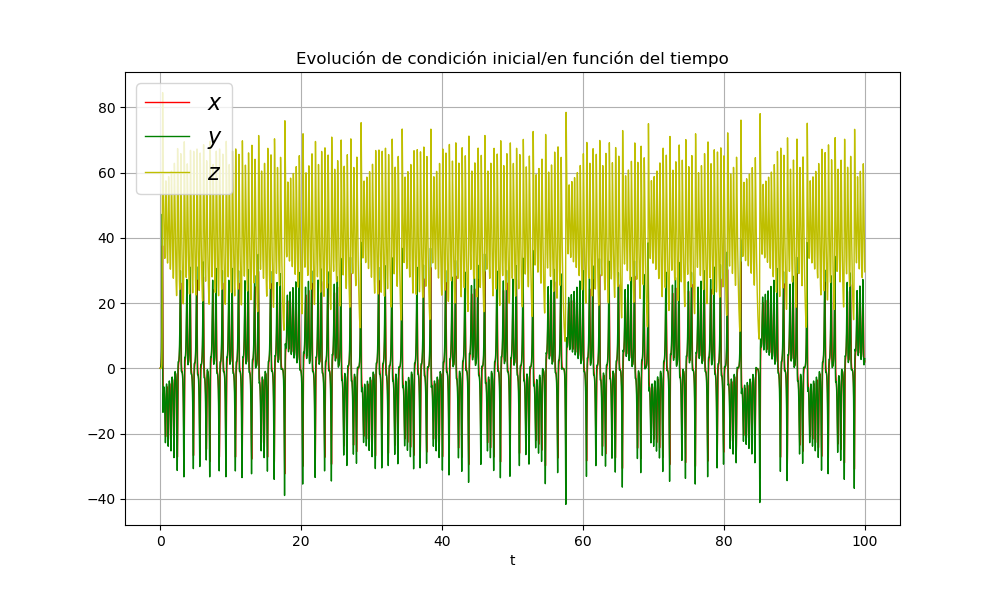
\includegraphics[scale = 0.65]{Evolucion2.png}
  \caption{Evolucion de cada variable respecto al tiempo}
\end{centering}
\end{figure}

\subsection{Sigma=10, Beta=8/3, Rho=99.92}

\begin{figure}
\begin{centering}
  \includegraphics[scale = 0.5]{lorenz-attractor-3d-3.png}
  \caption{Atractor de Lorenz}
\end{centering}
\end{figure}

\begin{figure}
\begin{centering}
  \includegraphics[scale = 0.4]{lorenz-attractor-phase-plane-3.png}
  \caption{Vista de los planos ortogonales del atractor de 2D}
\end{centering}
\end{figure}

\begin{figure}
\begin{centering}
  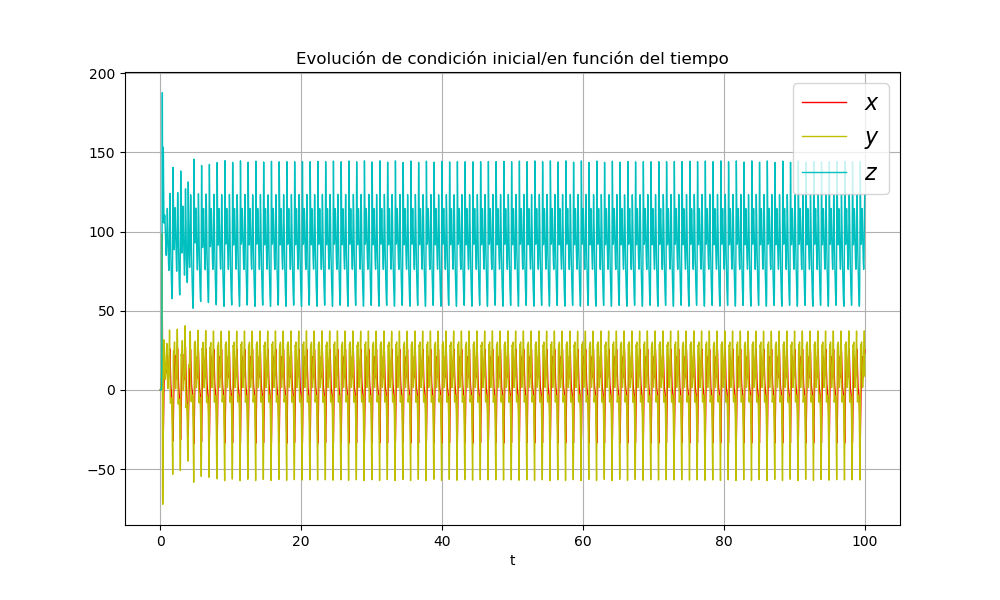
\includegraphics[scale = 0.65]{Evolucion3.png}
  \caption{Evolucion de cada variable respecto al tiempo}
\end{centering}
\end{figure}

\section{Bibliografía}

\begin{verbatim}
-Atractor de Lorenz(2018) De Wikipedia.org. Recopilado el 26 de Abril del 2018: https://es.wikipedia.org/wiki/Atractor_de_Lorenz

-J. Leys, E. Ghys, A. Alvarez.(2018) Caos VII: Atractores extraños. Recopilado el 26 de Abril del 2018: http://www.chaos-math.org/es/caos-vii-atractores-extranos


\end{verbatim}


\end{document}
